\documentclass[ecta]{econsocart}
\usepackage{amsmath,amssymb,booktabs,natbib,pdfpages,hyperref}
\hypersetup{hidelinks,hypertexnames=false,pdftitle={Neural Bellman Operators -- R11 Preservation Supplement},pdfauthor={Qian QI}}
\DeclareFontShape{T1}{ptm}{m}{uc}{<->ssub * ptm/m/sc}{}
\DeclareFontShape{T1}{ptm}{m}{up}{<->ssub * ptm/m/n}{}
\DeclareFontShape{T1}{ptm}{m}{scit}{<->ssub * ptm/m/it}{}
\begin{document}
\begin{frontmatter}
\title{Neural Bellman Operators: Preservation Supplement to Revision R11}
\runtitle{NBO: R11 Preservation Supplement}
\begin{aug}
\author[id=au1,addressref={add1}]{\fnms{Qian}~\snm{QI}\ead[label=e1]{qiqian@pku.edu.cn}}
\address[id=add1]{\orgname{Peking University}}
\end{aug}
\begin{abstract}
This supplement preserves the complete preceding R10 paper and its entire preservation supplement without deleting equations, proofs, numerical tables, or unsuccessful calculations. The current manuscript is ECTA\_R11. Earlier precision and comparative-performance statements are dated results, not new claims. The R11 revision adds a frozen method-specific tuning study, independent holdout evidence, exact continuous reference calculations, implemented-output error identities, and executed absolute-accuracy frontiers. All historical source files remain unchanged.
\end{abstract}
\end{frontmatter}
\section*{Reading map}
The R11 manuscript contains the original economy, all R10 main results and proofs, the added method-specific tuning study, the full absolute-accuracy calculations, and their verification details. A separate point-by-point response identifies the changes against every finding of the latest R9 referee report. The immutable source, result, build, and review identities are recorded in the revision directory.

The following pages reproduce the complete R10 manuscript. They are followed by the complete R10 supplement, which already preserves R9, R8, and earlier development material. In particular, recursive utility, sophisticated temporal selves, games, stochastic traces, action safeguards, unsuccessful earlier certificates, and all retained external experiments remain available. These earlier documents must be read with their original version labels. R11 does not turn an earlier failed tolerance or an exploratory numerical result into a current certificate merely by reproducing it.

\section*{Part I: Complete R10 manuscript}
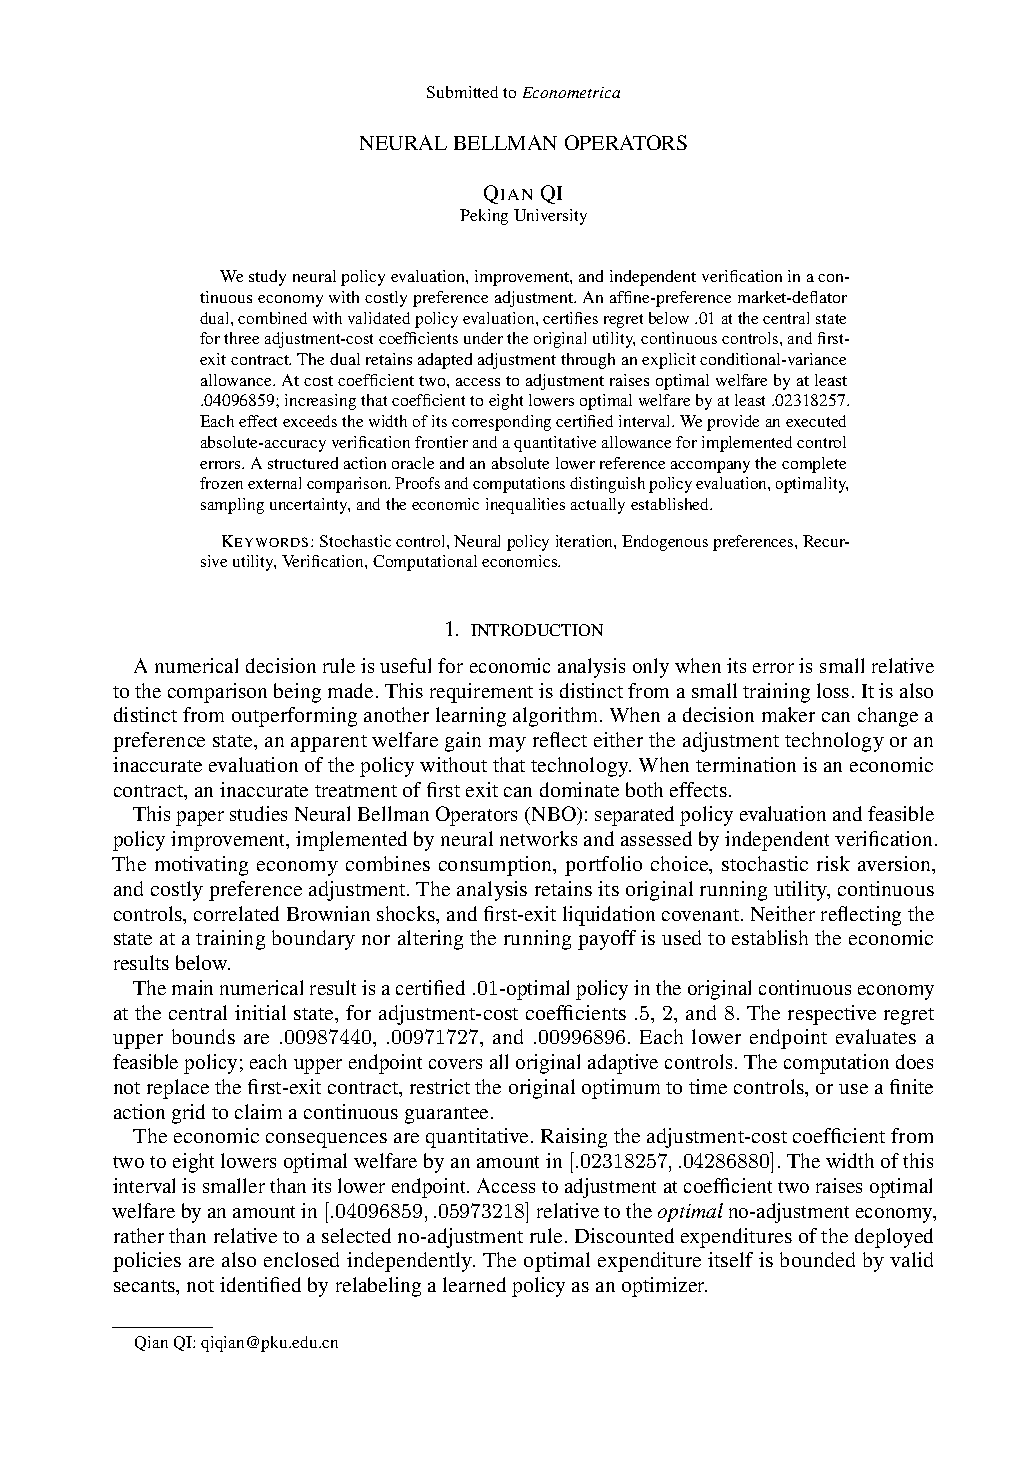
\includepdf[pages=-,pagecommand={},fitpaper=true]{ECTA_R10.pdf}
\section*{Part II: Complete R10 preservation supplement}
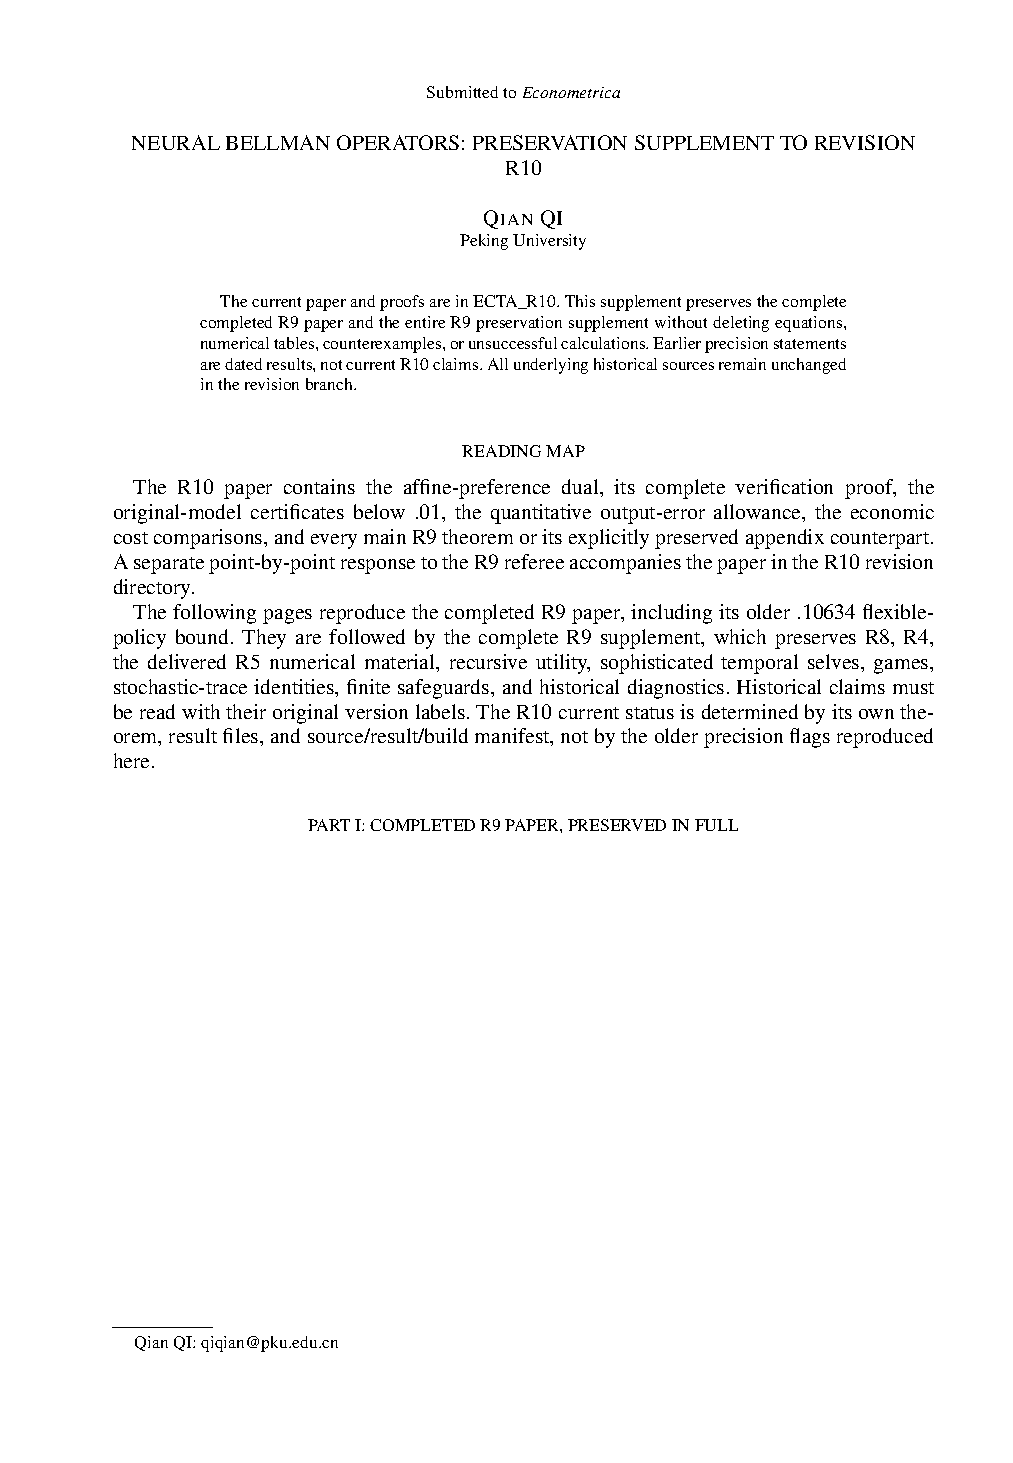
\includepdf[pages=-,pagecommand={},fitpaper=true]{SUPP_R10.pdf}
\end{document}
